% !TEX program = lualatex
% !BIB program = biber

% ==============================================================================
% Tutorial: Animation
% ==============================================================================
% \pause: for generally reveal items
% \item<1->\n \item<2->: similar to pause, display items one by one. 
% \only<1>{content}: only show content in slide no. 1. For replacing items in next slide. 

% ==============================================================================
% Tutorial: Fonts
% ==============================================================================
% math font: 
% 	\usefonttheme[onlymath]{serif}: use serif style math font

% ==============================================================================
% Tutorial: Block environment
% ==============================================================================
% Three blocks: 
% 	block
% 	alertblock
% 	exampleblock
% \begin{block}{title}
% 	content
% \end{block}
% \metroset{block=fill}: use background color, if not, the background is white. 

% ==============================================================================
% Tutorial: Sign and symbols
% ==============================================================================
% \setbeamertemplate{section in toc}[square]: set symbols in front of a section in table of content. 

\documentclass[8pt,dvipsnames,table]{beamer}

% ==============================================================================
% Language and Encoding
% ==============================================================================
\usepackage[utf8]{inputenc}
\usepackage[english]{babel}
% \usepackage[square,sort]{natbib}
\usepackage[backend=biber,style=apa]{biblatex}

% ------------------------------------------------------------------------------
% Citation
% ------------------------------------------------------------------------------
% \usepackage[square]{natbib}
% Usage: 
	% \citet no parenthesis
	% \citep with parenthesis
	% square option for square bracket
	% round option for round parenthesis

% ==============================================================================
% BibLaTeX configuration
% ==============================================================================
\addbibresource{../Bib.bib}
\DeclareLanguageMapping{american}{american-apa}

% ==============================================================================
% Font
% ==============================================================================
% \usefonttheme{professionalfonts}
% \usefonttheme{serif}
% \usepackage[T1]{fontspec}
% \setmainfont{Helvetica Neue}
\usepackage[scaled]{helvet}
\usepackage{lmodern}
% \usepackage{fourier}
% \usepackage{kmath}
% \usepackage[OT1]{eulervm}
\usefonttheme[onlymath]{serif}

% ==============================================================================
% Color, style and layout
% ==============================================================================
\usepackage{xcolor}
\usepackage{graphicx}
\usepackage[export]{adjustbox}
\usepackage{bm}
\usepackage{subfig}
\usepackage{pict2e}
\usepackage{comment}
\usepackage{pdfpages}
\usepackage{geometry}
% \usepackage[paper=landscape]{typearea}
\usepackage[makeroom]{cancel}
% \usepackage{arev}

% ==============================================================================
% Math and Physics
% ==============================================================================
\usepackage{mathrsfs}
\usepackage{physics}
\usepackage{slashed}
\usepackage{siunitx}
\usepackage{tikz-feynman}

% ==============================================================================
% Beamer backup
% ==============================================================================
\usepackage{appendixnumberbeamer}

% ==============================================================================
% Theme
% ==============================================================================
\usetheme{metropolis}
% \usecolortheme[snowy]{owl}
\linespread{1.5}

% ==============================================================================
% ifthen for User-definition
% ==============================================================================
\usepackage{ifthen}
% HOWTO:
% \ifthenelse{<test>}{<code for true>}{<code for false>}

% ==============================================================================
% Macros
% ==============================================================================
%\newcommand{\phanitem}{\phantom{\item}}
% \newcommand{\lag}{\mathcal{L}}
% \newcommand{\Mcal}{\mathcal{M}}
% \newcommand{\g}{\gamma}
% \renewcommand{\a}{\alpha}
% \newcommand{\s}{\sigma}
% \newcommand{\calA}{\mathcal{A}}
\newcommand{\mm}[1]{\frac{\dd^4#1}{(2\pi)^4}}
\newcommand{\mme}[1]{\frac{\dd^3\vb{#1}}{(2\pi)^3}}
\newcommand{\mmd}[2][d]{\ifthenelse{\equal{#1}{1}}{\frac{\dd {#2}}{2\pi}}{\frac{\dd^{#1}{#2}}{(2\pi)^{#1}}}}

% ==============================================================================
% Color Command
% ==============================================================================
% \definecolor{red}{rgb}{1, 0., 0.}

\newcommand{\red}[1]{{\color{OrangeRed}#1}}
\newcommand{\orange}[1]{{\color{Bittersweet}#1}}
\newcommand{\blue}[1]{{\color{NavyBlue}#1}}
\newcommand{\green}[1]{{\color{ForestGreen}#1}}
\newcommand{\purple}[1]{{\color{RedViolet}#1}}

% ==============================================================================
% Itemize style
% ==============================================================================
\setbeamertemplate{itemize item}{$\square$}
\makeatletter
\renewcommand{\itemize}[1][]{%
	\beamer@ifempty{#1}{}{\def\beamer@defaultospec{#1}}%
	\ifnum \@itemdepth >2\relax\@toodeep\else
	\advance\@itemdepth\@ne
	\beamer@computepref\@itemdepth% sets \beameritemnestingprefix
	\usebeamerfont{itemize/enumerate \beameritemnestingprefix body}%
	\usebeamercolor[fg]{itemize/enumerate \beameritemnestingprefix body}%
	\usebeamertemplate{itemize/enumerate \beameritemnestingprefix body begin}%
	\list
	{\usebeamertemplate{itemize \beameritemnestingprefix item}}
	{\def\makelabel##1{%
			{%
				\hss\llap{{%
						\usebeamerfont*{itemize \beameritemnestingprefix item}%
						\usebeamercolor[fg]{itemize \beameritemnestingprefix item}##1}}%
			}%
		}%
	}
	\fi%
	\setlength\itemsep{\fill}
	\ifnum \@itemdepth >1
	\vfill
	\fi%  
	\beamer@cramped%
	\raggedright%
	\beamer@firstlineitemizeunskip%
}
\def\enditemize{\ifhmode\unskip\fi\endlist%
	\usebeamertemplate{itemize/enumerate \beameritemnestingprefix body end}
	\ifnum \@itemdepth >1
	\vfil
	\fi%  
}
\makeatother
% \setbeamerfont{itemize/enumerate body}{size=\large}
% \setbeamerfont{itemize/enumerate subbody}{size=\normalsize}
% \setbeamerfont{itemize/enumerate subsubbody}{size=\small}


% ==============================================================================
% Horizontal Alignment
% ==============================================================================
\makeatletter
\newcommand{\pushright}[1]{\ifmeasuring@#1\else\omit\hfill$\displaystyle#1$\fi\ignorespaces}
\newcommand{\pushleft}[1]{\ifmeasuring@#1\else\omit$\displaystyle#1$\hfill\fi\ignorespaces}
\makeatother

% ==============================================================================
% Graphics Path
% ==============================================================================
\graphicspath{{./}}

% ==============================================================================
% Tikz Settings
% ==============================================================================
\tikzfeynmanset{
	with arrow/.style={
		/tikz/decoration={
				markings,
				mark=at position #1 with {
					\node[
					transform shape,
					xshift=-0.1mm,
					fill,
					dart tail angle=120,
					inner sep=0.7pt,
					draw=none,
					dart
					] { };
				},
			},
		/tikz/postaction={
			/tikz/decorate=true,
		},
	},
	with reversed arrow/.style={
		/tikz/decoration={
				markings,
				mark=at position #1 with {
					\node[
					transform shape,
					xshift=-0.1mm,
					rotate=180,
					fill,
					dart tail angle=120,
					inner sep=0.7pt,
					draw=none,
					dart
					] { };
				},
			},
		/tikz/postaction={
			/tikz/decorate=true,
		},
	}
}

% ==============================================================================
% Tikz Externalization
% ==============================================================================
% \usepackage{shellesc}
% \usetikzlibrary{external}
% % \usepgfplotslibrary{external}
% \tikzexternalize[shell escape=-enable-write18,prefix=./,system call={lualatex \tikzexternalcheckshellescape -halt-on-error -interaction=batchmode -jobname "\image" "\texsource"},up to date check=md5]
% \usepackage{luatexja-fontspec}
% \setmainjfont{wqy-zenhei}
% ==============================================================================
% Title Page
% ==============================================================================
\title{Annual Assessment Report}
\author[Y. Huang]{Yingsheng Huang (Supervisor: Yu Jia)}
\institute[IHEP]{Institute of High Energy Physics}
\date{\today}

\metroset{block=fill}
\setbeamertemplate{section in toc}[square]


\begin{document}

\begin{frame}{}
	\maketitle
	% \par\medskip
	% \uncover<4->{\vsapce*{-3in}arxiv:1809.09023}
\end{frame}

\begin{frame}
	\frametitle{Outlines}
	\tableofcontents
\end{frame}

\section{Operator Product Expansion for Atomic Wave-functions}
\begin{frame}
	\frametitle{Motivation}

	
	\begin{itemize}
		\item \red{Universal behaviors} in Coulombic wave-functions, \orange{near-origin} \green{divergence} in relativistic wave-functions (i.e. Hydrogen atom, Taylor expanded): 
	\end{itemize}
	\begin{align*}
		R^{\textrm{Schr}}_{n0}(r) & \propto
		\begin{cases}
			\arraycolsep=1.4pt\def\arraystretch{1.5}
			\begin{array}{lrll}
				1-\red{\dfrac{r}{a_0}}+ & \frac{1}{2} \blue{\dfrac{r^2}{a_0^2}}   & +\cdots & (n=1) \\
				1-\red{\dfrac{r}{a_0}}+ & \frac{3}{8} \blue{\dfrac{r^2}{a_0^2}}   & +\cdots & (n=2) \\
				1-\red{\dfrac{r}{a_0}}+ & \frac{19}{54} \blue{\dfrac{r^2}{a_0^2}} & +\cdots & (n=3) \\
				1-\red{\dfrac{r}{a_0}}+ & \frac{11}{32} \blue{\dfrac{r^2}{a_0^2}} & +\cdots & (n=4) \\
			\end{array}
		\end{cases},\\
		\only<1>{R^{\textrm{KG}}_{n0}(r)   & \propto
		\begin{cases}
			\arraycolsep=1.4pt\def\arraystretch{1.5}
			\begin{array}{lrll}
				1 -\red{\dfrac{r}{a_0}}     + & \frac{1}{2} \blue{\dfrac{r^2}{a_0^2}}   & -\orange{Z^2\alpha^2 \log{\left(\dfrac{r}{a_0}\right)}}+\green{Z^2\alpha^2 \left(\dfrac{r}{a_0}\right)\log{\left(\dfrac{r}{a_0}\right)}}+\cdots & \hspace{-5pt} (n=1) \\
				1 -\red{\dfrac{r}{a_0}}     + & \frac{3}{8} \blue{\dfrac{r^2}{a_0^2}}   & -\orange{Z^2\alpha^2 \log{\left(\dfrac{r}{a_0}\right)}}+\green{Z^2\alpha^2 \left(\dfrac{r}{a_0}\right)\log{\left(\dfrac{r}{a_0}\right)}}+\cdots & \hspace{-5pt} (n=2) \\
				1 -\red{\dfrac{r}{a_0}}    +  & \frac{19}{54} \blue{\dfrac{r^2}{a_0^2}} & -\orange{Z^2\alpha^2 \log{\left(\dfrac{r}{a_0}\right)}}+\green{Z^2\alpha^2 \left(\dfrac{r}{a_0}\right)\log{\left(\dfrac{r}{a_0}\right)}}+\cdots & \hspace{-5pt} (n=3) \\
				1 -\red{\dfrac{r}{a_0}}   +   & \frac{11}{32} \blue{\dfrac{r^2}{a_0^2}} & -\orange{Z^2\alpha^2 \log{\left(\dfrac{r}{a_0}\right)}}+\green{Z^2\alpha^2 \left(\dfrac{r}{a_0}\right)\log{\left(\dfrac{r}{a_0}\right)}}+\cdots & \hspace{-5pt} (n=4) \\
			\end{array}
		\end{cases}}
		\only<2>{
			R^{\textrm{Dirac}}_{n0}  (r) &\propto
		\begin{cases}
			\arraycolsep=1.4pt\def\arraystretch{1.5}
			\begin{array}{lrllll}
				1-\red{\dfrac{r}{a_0}}+       & \frac{1}{2} \blue{\dfrac{r^2}{a_0^2}}   & -\purple{\bm{\dfrac{1}{2}}}\orange{Z^2\alpha^2 \log{\left(\dfrac{r}{a_0}\right)}} & +  \purple{\bm{\dfrac{1}{2}}}\green{Z^2\alpha^2 \left(\dfrac{r}{a_0}\right)\log{\left(\dfrac{r}{a_0}\right)}} & +\cdots & \hspace{-5pt}  (n=1) \\
				1 -\red{\dfrac{r}{a_0}}     + & \frac{3}{8} \blue{\dfrac{r^2}{a_0^2}}   & -\purple{\bm{\dfrac{1}{2}}}\orange{Z^2\alpha^2 \log{\left(\dfrac{r}{a_0}\right)}} & +  \purple{\bm{\dfrac{1}{2}}}\green{Z^2\alpha^2 \left(\dfrac{r}{a_0}\right)\log{\left(\dfrac{r}{a_0}\right)}} & +\cdots & \hspace{-5pt} (n=2)  \\
				1 -\red{\dfrac{r}{a_0}}    +  & \frac{19}{54} \blue{\dfrac{r^2}{a_0^2}} & -\purple{\bm{\dfrac{1}{2}}}\orange{Z^2\alpha^2 \log{\left(\dfrac{r}{a_0}\right)}} & +  \purple{\bm{\dfrac{1}{2}}}\green{Z^2\alpha^2 \left(\dfrac{r}{a_0}\right)\log{\left(\dfrac{r}{a_0}\right)}} & +\cdots & \hspace{-5pt} (n=3)  \\
				1 -\red{\dfrac{r}{a_0}}   +   & \frac{11}{32} \blue{\dfrac{r^2}{a_0^2}} & -\purple{\bm{\dfrac{1}{2}}}\orange{Z^2\alpha^2 \log{\left(\dfrac{r}{a_0}\right)}} & +  \purple{\bm{\dfrac{1}{2}}}\green{Z^2\alpha^2 \left(\dfrac{r}{a_0}\right)\log{\left(\dfrac{r}{a_0}\right)}} & +\cdots & \hspace{-5pt} (n=4)  \\
			\end{array}
		\end{cases}
		}
	\end{align*}

\end{frame}

\begin{frame}
	\frametitle{Attack the problem with OPE \& EFT: Construct EFT}

	
	\begin{itemize}
		\item Use \green{\bf non-relativistic QED (NRQED)} for electron and \purple{\bf heavy nucleus effective theory (HNET, similar to HQET)} for nucleus\only<2>{, \red{\bf keep only Coulomb potential}}. 
		\item Lagrangian for non-relativistic atoms:
		\begin{align}
			\mathcal{L}= \only<1>{{\cal L}_{\rm Max}}\only<2>{\bcancel{{\cal L}_{\rm Max}}\;\red{\mathcal{L}_{\rm Coul}}}+ {\cal L}_{\rm NRQED} +{\cal L}_{\rm HNET} + \delta {\cal L}_{\rm contact}
			\label{LAGFULL}
		\end{align}
		where
		\begin{align*}
			  & \only<1>{{\cal L}_{\rm Max}= -\frac{1}{4} d_\gamma F_{\mu\nu}F^{\mu\nu}+\cdots, }\only<2>{\red{{\cal L}_{\rm Coul}= 
			  \frac{1}{2} \left(\nabla A^0\right)^2}},                             \\
			  & {\cal L}_{\rm NRQED}={\psi^\dagger \Bigg\{\red{iD_0+ {{\bf D}^2 \over 2m}} + \orange{ {{\bf D}^4\over 8m^3}+c_D e
			  {[\bm\nabla\cdot {\bf E}]\over 8m^2}}+\cdots\Bigg\}},\\
			%   c_D e
				% {[\bm\nabla\cdot {\bf E}]\over 8m^2}+c_F e {{\bm\sigma}\cdot{\bf B}\over 2m}+ ic_S e {({\bf D}\times {\bf E}-{\bf E}\times {\bf D})\cdot
			% \bm{\sigma}\over 8m^2}+\cdots\Bigg\}\psi,}\\
			  & {\cal L}_{\rm HNET}= \red{N^\dagger i D_0 N}+\cdots,                                                     \\
			  & \only<1>{\delta {\cal L}_{\rm contact}= {c_4\over m^2} \psi^\dagger\psi N^\dagger N+\cdots,}\only<2>{\xcancel{\delta {\cal L}_{\rm contact}= {c_4\over m^2} \psi^\dagger\psi N^\dagger N+\cdots,}}
		\end{align*}
		where $D^\mu=\partial^\mu+ieA^\mu$.
	\end{itemize}

\end{frame}

\begin{frame}
	\frametitle{Attack the problem with OPE \& EFT: OPE}

	\begin{itemize}
		\item Operator Product Expansion (OPE): The limit when product of local operators at different points approach each other.
				\begin{align}
					T\phi(x)\phi(0)\sim\sum_{\mathcal{O}}C_{\mathcal{O}}(x^{\mu})[\mathcal{O}(0)]_R
				\end{align}
	\end{itemize}
	\onslide<+->\metroset{block=fill}
	\begin{block}{\large Correct OPE relation in coordinate space}
		\begin{align*}
			\psi({\bf r})N({\bf 0})=(1-mZ\alpha |{\bf r}|)\,[\psi N]({\bf 0})
			+ (1-mZ\alpha |{\bf r}|/2){\bf r}\cdot [{\bf\nabla}\psi N]({\bf 0})+\cdots
			% \label{OPEME}
		\end{align*}
	\end{block}

	\begin{block}{\large Correct OPE relation in momentum space}
		\begin{align*}
			\widetilde\psi({\bf q})N({\bf 0}) & \equiv \int d^3 {\bf r}
			e^{-i {\bf q}\cdot {\bf r}} \psi({\bf r})N({\bf 0})\nonumber\\&= \frac{8\pi Z\alpha m}{{\bf q}^4} [\psi N]({\bf 0})-\frac{16 i \pi Z\alpha m}{{\bf q}^6}\bm{q}
			\cdot [{\bf\nabla}\psi N] ({\bf 0})+\cdots.
			% \label{OPEMEMOM}
		\end{align*}
	\end{block}
\end{frame}

% \begin{frame}
% 	\frametitle{Attack the problem with OPE \& EFT: OPE}

% 	\begin{itemize}
% 		\item Operator Product Expansion (OPE): The limit when product of local operators at different points approach each other.
% 		      \begin{align}
% 			      T\phi(x)\phi(0)\sim\sum_{\mathcal{O}}C_{\mathcal{O}}(x^{\mu})[\mathcal{O}(0)]_R
% 			  \end{align}
% 	\onslide<+->\item Naive expansion:
% 	\begin{align}
% 		\psi({\bf r})N({\bf 0})=[\psi N]({\bf 0})
% 		+ {\bf r}\cdot [{\bf\nabla}\psi N]({\bf 0})+\cdots
% 	\end{align}
% 	\onslide<+->$\Rightarrow$ This is wrong!!!

% 	\onslide<+->
% 	\hspace{1in}
% 	\begin{center}
% 		\orange{\Large\textbf{\textsc{We need to consider \underline{RADIATIVE CORRECTIONS}}}}
% 	\end{center} 

	
% 	\end{itemize}
% \end{frame}

% \begin{frame}
% 	\frametitle{Attack the problem with OPE \& EFT: OPE}

% 	\onslide<+->\metroset{block=fill}
% 	\begin{block}{\large Correct OPE relation in coordinate space}
% 		\begin{align*}
% 			\psi({\bf r})N({\bf 0})=(1-mZ\alpha |{\bf r}|)\,[\psi N]({\bf 0})
% 			+ (1-mZ\alpha |{\bf r}|/2){\bf r}\cdot [{\bf\nabla}\psi N]({\bf 0})+\cdots
% 			% \label{OPEME}
% 		\end{align*}
% 	\end{block}

% 	\begin{block}{\large Correct OPE relation in momentum space}
% 		\begin{align*}
% 			\widetilde\psi({\bf q})N({\bf 0}) & \equiv \int d^3 {\bf r}
% 			e^{-i {\bf q}\cdot {\bf r}} \psi({\bf r})N({\bf 0})\nonumber\\&= \frac{8\pi Z\alpha m}{{\bf q}^4} [\psi N]({\bf 0})-\frac{16 i \pi Z\alpha m}{{\bf q}^6}\bm{q}
% 			\cdot [{\bf\nabla}\psi N] ({\bf 0})+\cdots.
% 			% \label{OPEMEMOM}
% 		\end{align*}
% 	\end{block}

% \end{frame}

\begin{frame}
	\frametitle{Reproduce Wave-function origin}

	
	
	\begin{itemize}
		\item With operator definition of the wave-functions 
		\begin{align}
			\Psi_{nlm}({\bf r})=\left\langle 0\left\vert\psi({\bf r})N({\bf 0})\right\vert nlm \right\rangle
		\end{align}
	\begin{block}{\large Wave-function origin (Schr\"odinger equation)}
		\begin{align}
			& R_{n0}(r)= R_{n0}(0)
		  \left[1-{r\over a_0}+{\mathcal O}\left(r/a_0\right)^2\right]
		\end{align}
	\end{block}
	\item Add \orange{\bf relativistic corrections} in OPE with higher order Lagrangian to account for the logarithms in \orange{\bf relativistic wave-functions (Klein-Gordon, Dirac)}. 
	\item Use renormalization group equation to reproduce all leading logarithms. 
	\end{itemize}

\end{frame}

\section{Meson-meson Scattering in 1+1-d QCD}
\begin{frame}
	\frametitle{'t Hooft equation}

	
	\begin{minipage}{0.48\textwidth}
		\begin{itemize}
			\item Large-N Expansion
			\item In 1+1-d, \orange{\bf ONLY PLANAR DIAGRAM!!!}
		\end{itemize}
	Steps: 
	\begin{enumerate}
		\item \small Obtain mesons' 't Hooft wave-functions with 't Hooft equation (Fig~\ref{dressedquark}). 
		\item Obtain effective meson-meson vertex function with Bethe-Salpeter equation (Fig~\ref{BSequation}). 
		\item Calculate meson-meson scattering amplitude with said vertex functions and wave-functions. 
	\end{enumerate}
	\end{minipage}
	\begin{minipage}{0.48\textwidth}
		\begin{figure}[hbt]
			\begin{center}
			  % Requires \usepackage{graphicx}
			  \includegraphics[width=1\textwidth]{dressedquark.eps}\\
			  \caption{The Dyson-Schwinger equation for the quark self-energy. }\label{dressedquark}
			  \end{center}
		\end{figure}
		\begin{figure}[hbt]
			\begin{center}
			  % Requires \usepackage{graphicx}
			  \includegraphics[width=0.7\textwidth]{BS.eps}\\
			  \caption{The Bethe-Salpeter equation for the $q\bar{q}$ bound state.}\label{BSequation}
			  \end{center}
		\end{figure}
	\end{minipage}

	\vspace*{1mm}

	't Hooft equation
	\begin{equation}
		\mu^2
		\varphi(x)=\left(\frac{\alpha_{1}}{x}+\frac{\alpha_{2}}{1-x}\right)\varphi(x)-P\int_0^1
		dy\frac{\varphi(y)}{(x-y)^2}.\label{teq}
	\end{equation}
	$\mu$ is the mass of the meson, $\alpha_i$ is rescaled quark mass, $P$ marks principle value. 

\end{frame}
\begin{frame}
	\frametitle{Results \orange{(\textsc{No indication of tetraquark!!!})}}
	\vspace{-0.3in}
	\begin{figure}[!hbtp]
		\centering
			\subfloat[Amplitudes for the contact term in $A(c\bar c)+B(c\bar c)\rightarrow C(c\bar c)+D(c\bar c)$.]{
			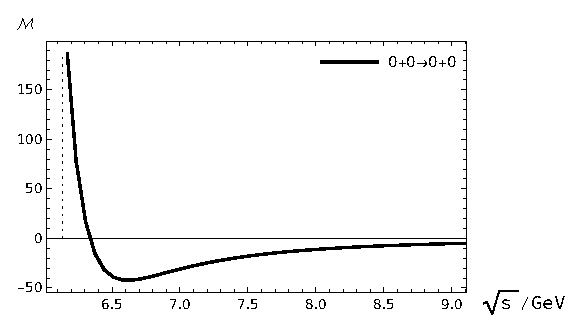
\includegraphics[width=0.49\textwidth]{1f.eps}
			% \caption{\small }
			\label{the1flavor}
			}\subfloat[Amplitudes for the contact term in $A(c\bar s)+B(c\bar s)\rightarrow C(c\bar s)+D(c\bar s)$.]{
			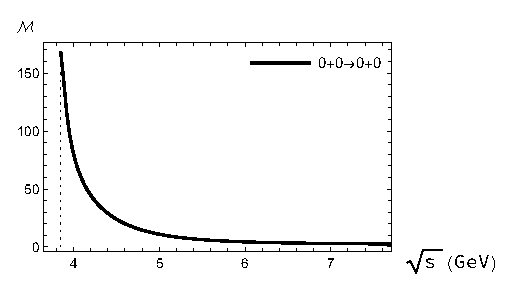
\includegraphics[width=0.49\textwidth]{2f.eps}
			% \caption{\small }
			\label{the1flavor}
			}\\ 
			
			\subfloat[Amplitudes for the contact term in $A(c\bar u)+B(c\bar d)\rightarrow C(c\bar u)+D(c\bar d)$.]{
			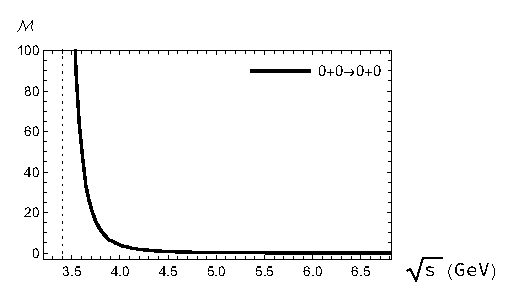
\includegraphics[width=0.49\textwidth]{3f.eps}
			% \caption{\small }
			\label{the1flavor}
			}
			\subfloat[Amplitudes for the contact term in $A(c\bar d)+B(b\bar s)\rightarrow C(b\bar d)+D(c\bar s)$ with particle B moving backwards. No near-threshold enhancement.]{
			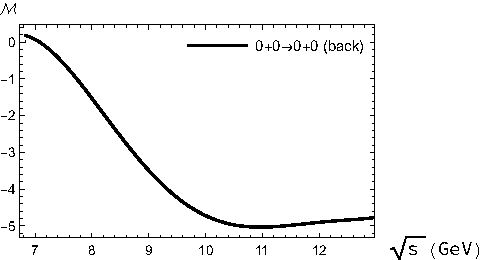
\includegraphics[width=0.49\textwidth]{4f.pdf}
			% \caption{\small }
			\label{the1flavor}
			}
	\end{figure}


\end{frame}

\section{Fragmentation Production of Fully-heavy Tetraquark at LHC}

\begin{frame}
	\frametitle{Factorization theorem for $T_{4c/b}$ production}

	\begin{itemize}
		\begin{minipage}{0.4\textwidth}
			\item {\tt LHCb} discovered a narrow structure near $6.9$ GeV in the di-$J/\psi$ invariant mass spectrum ($>5\sigma$): $X(6900)$.
			\item Strong candidate for fully-charmed tetraquark.
		\end{minipage}\hfill
		\begin{minipage}{0.5\textwidth}
			\begin{figure}
				\centering
				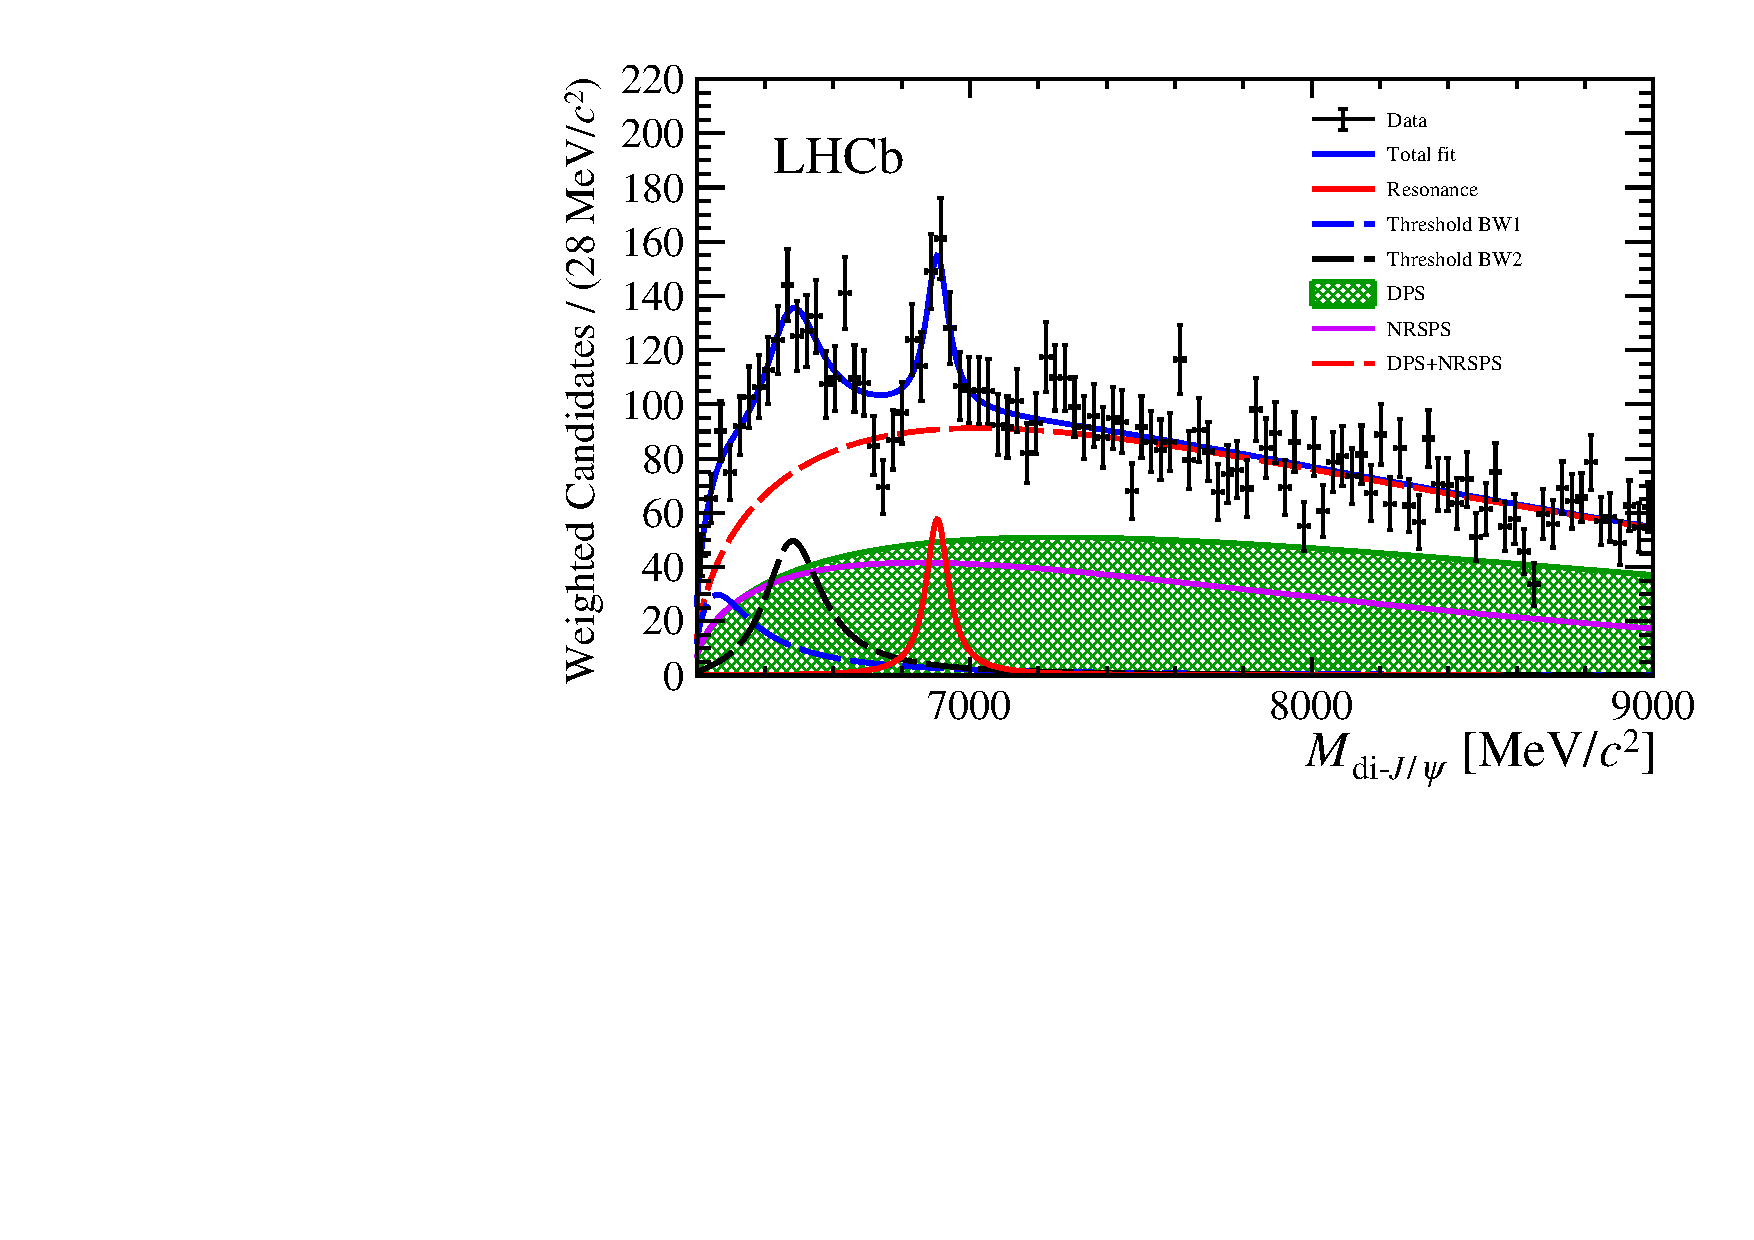
\includegraphics[width=\textwidth,frame]{Fig3b.pdf}
			\end{figure}
		\end{minipage}
		\item QCD factorization theorem for fully-heavy tetraquark ($T_{4c/b}$) exclusive production at high-$p_T$
		\begin{align}
			\mathrm{d} \sigma\left(p p \rightarrow T_{4c/b}\left(p_{\mathrm{T}}\right)+X\right) &=\sum_{i}\int_0^1 \mathrm{d} x_a  \int_0^1 \mathrm{d} x_b \int_{0}^{1} \mathrm{d} z\; f_{a/p}(x_a,\mu)f_{b/p}(x_b,\mu) \notag\\
			\times  \dd &{\hat \sigma}(a b \rightarrow i(p_T/z)+X, \mu)  D_{i \rightarrow T_{4c/b}}\left(z,\mu\right)+{\cal O}(1/p_T). 
			%-----------------------------------
			\label{QCD:fact:theor}
		\end{align}
		\item Dominate partonic channel is $gg\to gg$, rather than $gg\to q\bar{q}$. 
	\end{itemize}

\end{frame}

\begin{frame}
	\frametitle{Fragmentation Function}

	Collins-Soper definition of fragmentation function: 
	{\footnotesize
	\begin{align*}
		\begin{aligned}[b]
			&D_{g \rightarrow T_{4c}}(z, \mu)= \frac{-g_{\mu \nu} z^{d-3}}{2 \pi k^{+}\left(N_{c}^{2}-1\right)(d-2)} \int_{-\infty}^{+\infty} d x^{-} e^{-i k^{+} x^{-}}
			\\
			&\times\sum_X \left\langle 0\left|G_{c}^{+\mu}(0) \mathcal{E}^{\dagger}\left(0,0, \mathbf{0}_{\perp}\right)_{c b}
			|T_{4c}(P)+X\rangle\langle T_{4c}(P)+X| \mathcal{E}\left(0, x^{-}, \mathbf{0}_{\perp}\right)_{b a} G_{a}^{+\nu}\left(0, x^{-}, \mathbf{0}_{\perp}\right)\right| 0\right\rangle
			\label{CS:def:gluon:T4c:frag}
		\end{aligned}
	\end{align*}}
	\begin{minipage}{0.49\textwidth}
		{\small\begin{itemize}
			\item NRQCD factorization: 
			\begin{align*}
				D_{g \rightarrow H}(z)=\sum_{n} d_{n}(z)\left\langle 0\left|\mathcal{O}_{n}^{H}\right| 0\right\rangle
			\end{align*}
			\item Perturbative matching to determine short distance coefficients. 
			\item Use wave-function origin (S-wave) from potential models to determine long range matrix elements in order to yield a phenomenological result. 
			\item More details in Jia-Yue Zhang's talk this afternoon. 
		\end{itemize}}
	\end{minipage}\hfill
	\begin{minipage}{0.45\textwidth}
		\begin{figure}[hbtp]
			\centering
			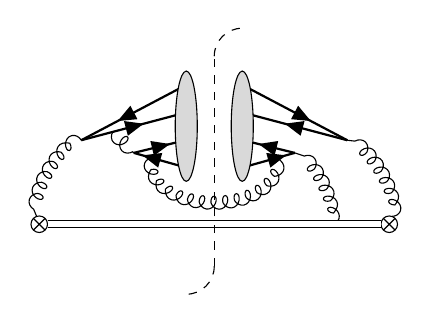
\begin{tikzpicture}[transform shape,scale=0.7]
				\begin{feynman}
					\node[crossed dot] (a);
					\node[right=2.5in of a,crossed dot] (b);
					\vertex at ($(a)+(0.3in,0.6in)$) (v1);
					\vertex at ($(b)+(-0.3in,0.6in)$) (v2);
					\vertex at ($(a)!0.5!(b)$) (o);
					\vertex at ($(o)+(-0.2in,0.7in)$) (o1);
					\vertex at ($(o)+(0.2in,0.7in)$) (o2);
					\vertex at ($(o1)+(0in,1cm)$) (end1);
					\vertex at ($(o1)+(0in,-1cm)$) (end2);
					\vertex at ($(end1)!0.125!(end2)$) (f1);
					\vertex at ($(end1)!0.375!(end2)$) (f2);
					\vertex at ($(end1)!0.625!(end2)$) (f3);
					\vertex at ($(end1)!0.875!(end2)$) (f4);
					\vertex at ($(v1)!0.3!(f2)$) (i1);
					\vertex at ($(i1)+(0.15in,-0.15in)$) (i2);
					\vertex at ($(o2)+(0in,1cm)$) (end11);
					\vertex at ($(o2)+(0in,-1cm)$) (end12);
					\vertex at ($(end11)!0.125!(end12)$) (f11);
					\vertex at ($(end11)!0.375!(end12)$) (f12);
					\vertex at ($(end11)!0.625!(end12)$) (f13);
					\vertex at ($(end11)!0.875!(end12)$) (f14);
					\vertex at ($(v2)!0.3!(f12)$) (i11);
					\vertex at ($(i11)+(-0.15in,-0.15in)$) (i12);
					\vertex at ($(o)!0.66!(b)$) (t1);
					\vertex at ($(i2)!0.33!(f4)$) (t2);
					\vertex at ($(i12)!0.33!(f14)$) (t3);
					\diagram*{
						(v1) --[gluon,quarter right, looseness=0.7] (a);
						(b) --[gluon,quarter right, looseness=0.7] (v2);
						(v1) --[anti fermion, thick] (f1);
						(v1) --[fermion, thick] (f2);
						(i1) --[gluon] (i2);
						(i2) --[fermion, thick] (f3);
						(i2) --[anti fermion, thick] (f4);
						(v2) --[anti fermion, thick] (f11);
						(t1) --[gluon,quarter right, looseness=0.7] (i12);
						(v2) --[fermion, thick] (f12);
						(i12) --[fermion, thick] (f13);
						(i12) --[anti fermion, thick] (f14);
						(t2) --[gluon,half right, looseness=1.2] (t3);
						(a) --[double distance=2pt] (b);
					};
					\draw[fill=gray!30!white] (o1) ellipse (0.2cm and 1cm);
					\draw[fill=gray!30!white] (o2) ellipse (0.2cm and 1cm);
					\vertex at ($(o)+(0in,-0.3in)$) (cut1);
					\vertex at ($(o)+(0in,1.2in)$) (cut2);
					\vertex at ($(cut2)+(0.2in,0.2in)$) (cut11);
					\vertex at ($(cut1)+(-0.2in,-0.2in)$) (cut22);
					\draw[dashed] (cut1) -- (cut2);
					\draw[dashed] (cut2) to[out=90,in=180] (cut11);
					\draw[dashed] (cut1) to[out=270,in=0] (cut22);
				\end{feynman}
			\end{tikzpicture}
			\caption{A representative Feynman diagram for the fragmentation function of gluon into $T_{4c}$. The grey blob indicates
			the $C$-even tetraquark. Horizontal double line denotes the eikonal line.}
			\label{tetra-diagrams}
		\end{figure}
	\end{minipage}

\end{frame}

\begin{frame}
	\frametitle{Phenomenology for $T_{4c/b}$ production at LHC}

	% \begin{minipage}{0.24\textwidth}
	% 	\begin{itemize}
	% 		\item 
	% 	\end{itemize}
	% \end{minipage}
	\begin{minipage}{0.99\textwidth}
		\begin{figure}[!hbtp]
			\centering
			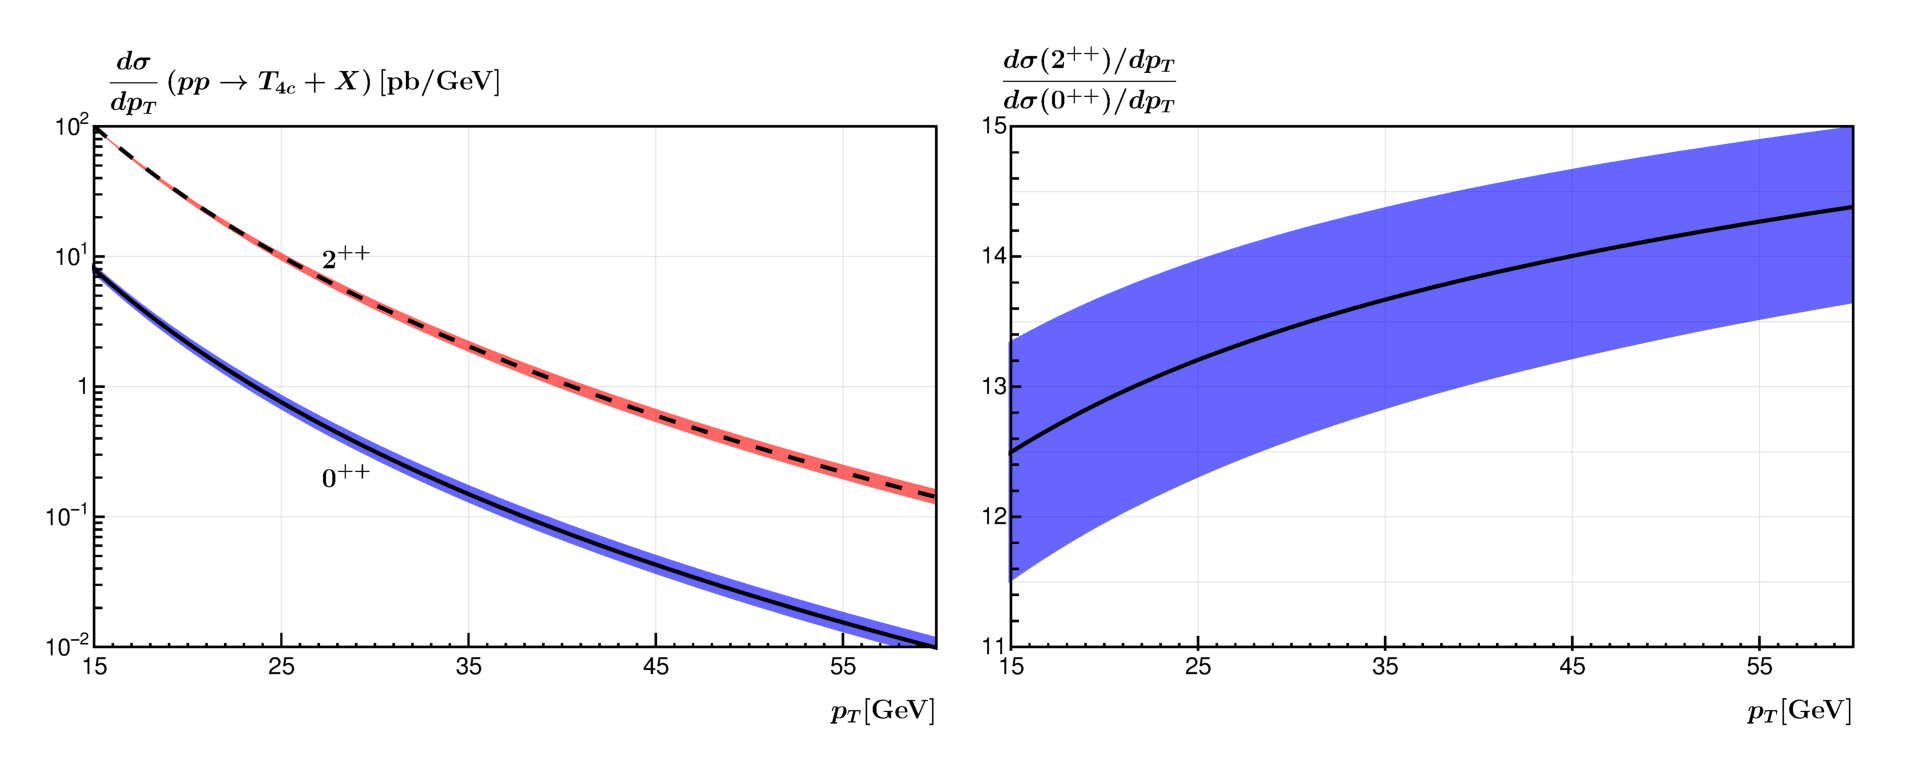
\includegraphics[width=\textwidth,frame]{cpTFig.eps}
			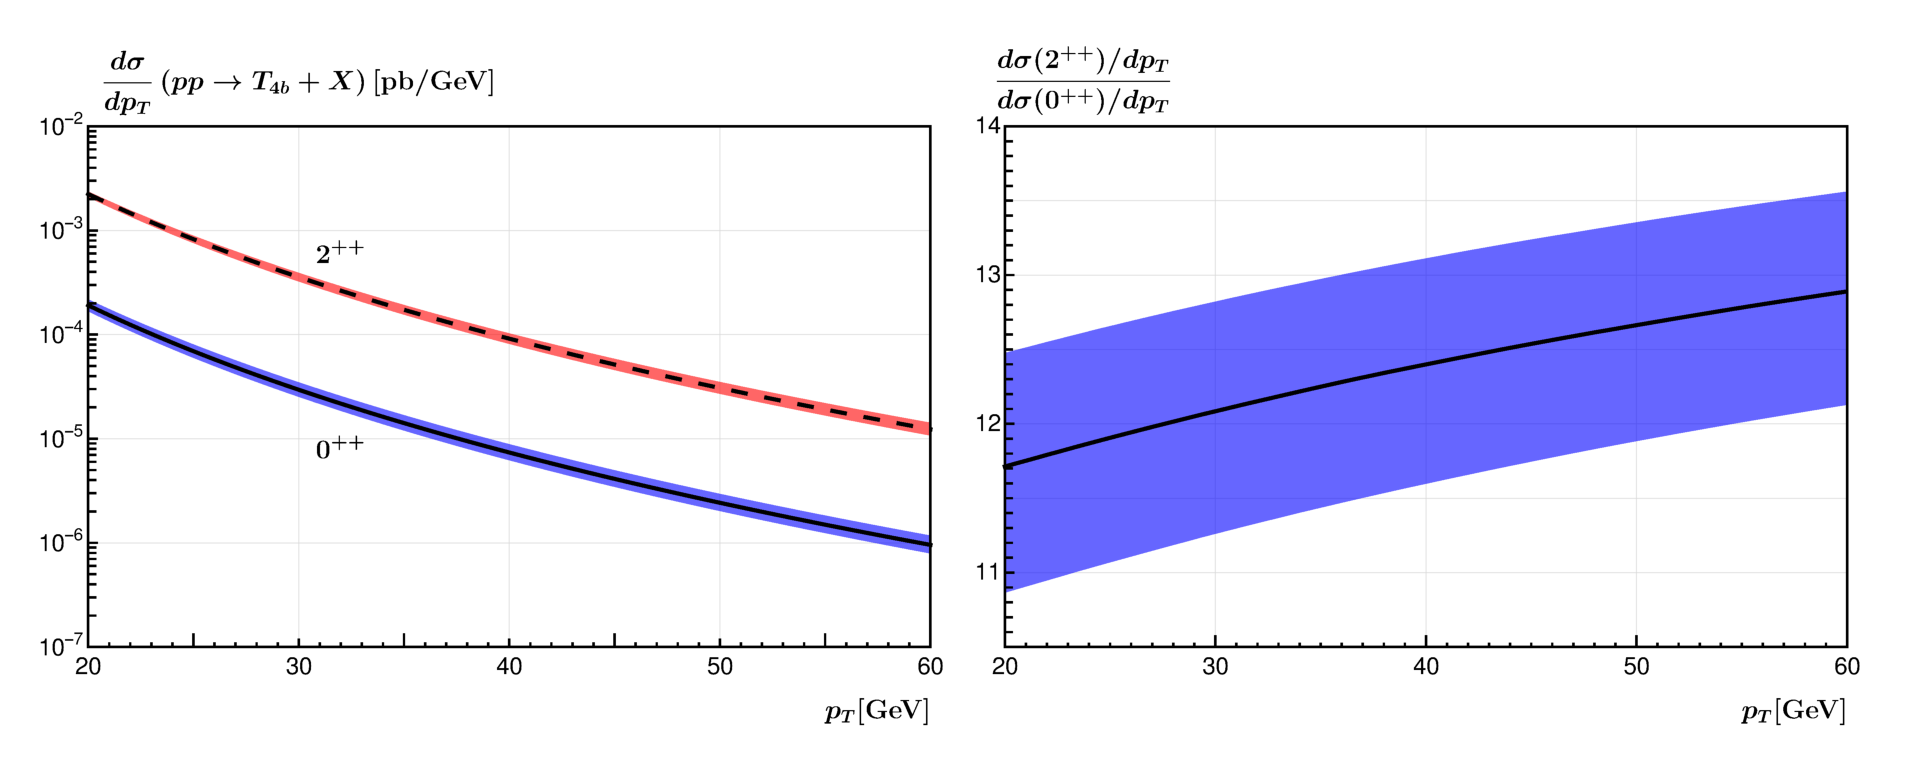
\includegraphics[width=\textwidth,frame]{bpTFig.eps}
			% \caption{The $p_T$ distribution of inclusive $T_{4c/4b}$ production on LHC. The central values (represented by the solid and dashed curves) are generated by setting $\mu=p_T$. The difference between $0^{++}$ and $2^{++}$ states are also given. }
			\label{fig:pT_dstrbtn}
		\end{figure}
	\end{minipage}

\end{frame}

\begin{frame}
	\frametitle{Phenomenology for $T_{4c/b}$ production at LHC}

	\begin{itemize}
		\item $2^{++}$ cross section is about 10 times larger than $0^{++}$. 
		\item We obtain the yields of the accumulated event number for $T_{4c}$ at HL-LHC are a hundred million for $0^{++}$ and 8 hundreds million for $2^{++}$ (with integrated luminosity 3000 $\rm{fb}^{-1}$). 
		\item The
		prediction for $T_{4b}$ is highly suppressed, mainly due to the relative larger bottom mass suppression.
		\item The total cross section we obtained is unreliable mainly due to the fact that fragmentation only works at high-$p_T$, and our integration is done within approximately $15\leq p_T\leq 60 \rm{GeV}$.
		% \begin{table}[h]
		% 	{\small\begin{tabular}{|c|c|c|c|c|c|}
		% 		\hline
		% 		&  & \multicolumn{2}{c|}{$0^{++}$} & \multicolumn{2}{c|}{$2^{++}$ }\tabularnewline
		% 		\hline
		% 		& $p_{T}$ range & $\sigma$  & $N_{\mathrm{events}}$ & $\sigma$  & $N_{\mathrm{events}}$\tabularnewline
		% 		\hline
		% 		$T_{4c}$ & $15\mathrm{\mathrm{GeV}}\leq p_{T}\leq60\mathrm{\mathrm{GeV}}$  & $33_{-4}^{+4}\mathrm{pb}$ & $9.9_{-1.2}^{+1.2}\times10^{7}$ & $424_{-21}^{+13}\mathrm{pb}$ & $1.27_{-0.06}^{+0.04}\times10^{9}$\tabularnewline
		% 		\hline
		% 		$T_{4b}$ & $20\mathrm{\mathrm{GeV}}\leq p_{T}\leq60\mathrm{\mathrm{GeV}}$  & $1.04_{-0.15}^{+0.17}\times10^{-3}\mathrm{pb}$ & $3.12_{-0.45}^{+0.51}\times10^{3}$ & $1.24_{-0.11}^{+0.11}\times10^{-2}\mathrm{pb}$ & $3.72_{-0.33}^{+0.33}\times10^{4}$\tabularnewline
		% 	\hline
		% 	\end{tabular}}
		% \caption{The $p_T$-integrated cross section for $T_4c$ inclusive production on LHC.}
		% \label{pT_intgrtd}
		% \end{table}
	\end{itemize}

\end{frame}

\section*{Publications}
\begin{frame}
	\frametitle{Publications?}

	
	{
	% \setbeamertemplate{itemize items}{$\arrowbullet$}
	\setbeamertemplate{itemize items}[triangle]
	\begin{itemize}
		\item\fullcite{Huang:2018yyf} {\bf (rejected by PRL, waiting for resubmission)}
		
		\item\fullcite{Huang:2018ils} {\bf (Submitted to PRD, referee comments received)}
		
		\item\fullcite{Huang:2019hdj} {\bf (rejected by PRL, waiting for appeal)}
	
		\item\fullcite{Chen2019} {\bf (Submitted to PRD and received positive response. )}
	
		\item\fullcite{Feng2020} {\bf (To be submitted to PRL)}
	\end{itemize}
	}

\end{frame}

\appendix
\begin{frame}[standout]
	\Huge Questions?
  \end{frame}
% \begin{frame}
% 	\begin{center}
% 		\Huge 
% 		\usebeamercolor[bg]{frametitle}
% 		\emph{Thanks for your attention!}
% 	\end{center}
% \end{frame}

\appendix
\begin{frame}
	\vfill
	\centering
	\begin{beamercolorbox}[sep=8pt,center,shadow=true,rounded=true]{title}
		\usebeamerfont{title}Backup\par%
	\end{beamercolorbox}
	\vfill
\end{frame}

\printbibliography

% \bibliography{../Bib}
% \bibliographystyle{apalike}

\end{document}
